%%%%%%%%%%%%%%%%%%%%%%%%%%%%%%%%%%%%%%%%%%%%%%%%%%%%%%%
%Anexo
%Este anexo foi incluido para explicar como incluir um anexo no estilo, não existia no original desta tese
%exceto algumas tabelas que foram modificadas
%%%%%%%%%%%%%%%%%%%%%%%%%%%%%%%%%%%%%%%%%%%%%%%%%%%%%%%%%%%%%%%%%%%%%%%%%%%%%%%%%
\renewcommand{\thechapter}{}%
\chapter{ANEXO B - EXEMPLOS DE FIGURAS E TABELAS NO \LaTeX} %% Título do anexo sempre em maiúsculas.
\label{anexoB} %% Rótulo aplicado caso queira referir-se a este tópico em qualquer lugar do texto.
\renewcommand{\thechapter}{B}%

\section{Figuras} %% Título de secção sempre com as primeiras letras em maiúsculas.
\label{anexo2}

\begin{figure}[ht]
	\caption{Exemplo de figura com título curto.}
	\vspace{6mm}	% acrescentar o espaçamento vertical apropriado entre o título e a borda superior da figura
	\begin{center}
    	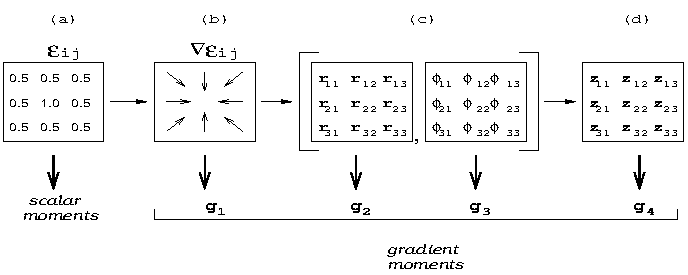
\includegraphics[width=\mylenfig]{./Figuras2/gpa.pdf}  
	\end{center}
	\vspace{4mm}	% acrescentar o espaçamento vertical apropriado entre a borda inferior da figura e a legenda ou a fonte quando não há legenda (o valor pode ser negativo para subir)
	\legenda{Exemplo de legenda curta.}	% legenda - opcional
	\label{figgpa1}
	\FONTE{\citeonline{lba/06}.}	% fonte consultada (elemento obrigatório, mesmo que seja produção do próprio autor)
\end{figure}

\begin{figure}[!h]
	\caption{Figura com título que ocupa mais de uma linha, alinhar as demais com a primeira
letra depois do hífen.}
%o ajuste do título é feito automaticamente pelo \LaTeX\ caso este ocupe mais de uma linha.}
	\vspace{6mm}	% acrescentar o espaçamento vertical apropriado entre o título e a borda superior da figura
	\begin{center}
    	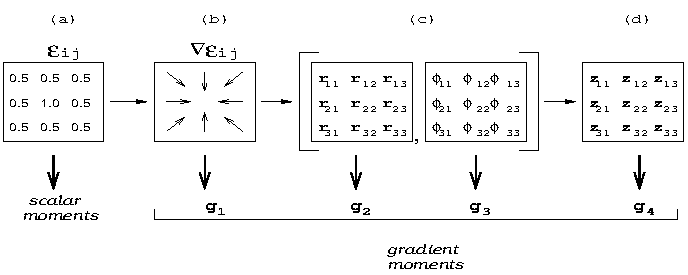
\includegraphics[width=\mylenfig]{./Figuras2/gpa.pdf}  
	\end{center}
	\vspace{4mm}	% acrescentar o espaçamento vertical apropriado entre a borda inferior da figura e a legenda ou a fonte quando não há legenda (o valor pode ser negativo para subir)
	\legenda{Exemplo de legenda que ocupa mais de uma linha, alinhar as demais com a primeira
letra da primeira linha.}	% legenda - opcional
%o \LaTeX\ alinha o texto automaticamente.
	\label{figgpa2}
	\FONTE{Se o texto da fonte for longo e ocupar mais de uma linha as demais ficam alinhadas
	com a palavra fonte. Adaptada de \citeonline{mauri:2003}.}	% fonte consultada (elemento obrigatório, mesmo que seja produção do próprio autor)
%o \LaTeX\ alinha o texto automaticamente.
\end{figure}

\clearpage
\section{Tabelas} 

\begin{table}[!ht]%[htbp] %opções de colocação da tabela no texto
  \begin{center}	% use sempre um ambiente para as tabelas
									% (opções: center (recomendado), flushright, flushleft)
									% NÃO USE \centering com TABELAS se houver \FONTE!	
  \caption{Exemplo de tabela, com fonte.}
    \begin{tabular}{l|l|c|c|r|r}
			\hline % desenha uma linha horizontal
				Campo 1 & Campo2 & Campo3 & Campo 4 & Campo5 & Campo6 \\
				Campo 1 & Campo2 & Campo3 & Campo 4 & Campo5 & Campo6 \\
				Campo 1 & Campo2 & Campo3 & Campo 4 & Campo5 & Campo6 \\				
			\hline % desenha uma linha horizontal
    \end{tabular}
    \end{center}
 \FONTE{Coloque a fonte de referência aqui, se houver.}
\end{table}

% \hhline{|--|} \multicolumn{2}{|c|}{continuação da página anterior} \\
% \hhline{|--|} \endhead % ate aqui eh definicao do "head" da pagina 
%   % dois em diante
% \hhline{|--|} \multicolumn{2}{|c|}{continua para próxima página} \\
% \hhline{|--|} \endfoot % ate aqui eh definicao do "foot" exceto ultima página
% \hhline{|b:=:=:b|} \endlastfoot % ate aqui eh definicao do "foot" 
%   % da ultima pagina

\begin{table}[hb]
\renewcommand{\baselinestretch}{1.4}% for tabular environment
\small
   \centering
   \caption{Exemplo de tabela, com fonte longa}
%   \label{\fullpaperid:table:1}% you must prefix your labels (here table:1) with the string \fullpaperid: (this will be important when combining all the full papers for the final book)
	\begin{center}
	   \begin{tabular}{lcc}
	       \hline% horizontal line
	       \itshape Parameter&
	           \itshape $\kappa$ Scaling&
	           \itshape $\kappa$, $\lambda$ Scaling\\*
	       \hline
	       Dimension&
	           $\kappa^{-1}$&
	           $\lambda^{-1}$\\*
	       Currant&
	           $\kappa^{-1}$&
	               $\lambda/\kappa^{2}$\\*
	       Dopant Concentration&
	           $\kappa$&
	           $\lambda2/\kappa$\\*
	       \hline
	   \end{tabular}
	\end{center}
    \renewcommand{\baselinestretch}{1.0}
    \FONTE{Coloque a fonte longa longa longa longa longa longa longa longa longa longa aqui, se houver.}
\end{table}

% Exemplos de 2 tabelas avançadas 

\begin{table}[ht!]
\caption{Outro exemplo de tabela}
%\label{\fullpaperid:table:2}
\begin{center}
\renewcommand{\baselinestretch}{1.2}% for tabular environment
\small
\begin{tabular}{cccccc}
\hline
   & \multirow{2}{22mm}{\renewcommand{\baselinestretch}{0.7}\small\centering Quantitative measures} & \multicolumn{4}{c}{Markers} \\ \cline{3-6}
   & & \multicolumn{1}{c}{RO} & \multicolumn{1}{c}{ASF} & \multicolumn{1}{c}{ISO} & \multicolumn{1}{c}{ADF} \\ \hline
   \multirow{3}{20mm}{\renewcommand{\baselinestretch}{0.7}\small\centering Test image scale 2}
& RMSE & 0.126 & 0.187 & 0.118 & 0.103 \\
& NMSE & 0.046 & 0.101 & 0.040 & 0.031 \\
& SSIM & 0.9981 & 0.9956 & 0.9984 & 0.9989 \\ \hline
   \multirow{3}{18mm}{\renewcommand{\baselinestretch}{0.7}\small\centering Cameraman scale 4}
& RMSE & 13.748 & 15.649 & 10.132 & 4.325 \\
& NMSE & 0.011 & 0.014 & 0.006 & 0.001 \\
& SSIM & 0.923 & 0.847 & 0.904 & 0.933 \\ \hline
   \multirow{3}{18mm}{\renewcommand{\baselinestretch}{0.7}\small\centering Cameraman scale 7}
& RMSE & 20.963 & 22.652 & 13.108 & 4.650 \\
& NMSE & 0.024 & 0.029 & 0.010 & 0.001 \\
& SSIM & 0.851 & 0.757 & 0.866 & 0.925 \\ \hline
   \multirow{3}{23mm}{\renewcommand{\baselinestretch}{1.2}\small\centering Crop of cameraman scale 7}
& RMSE & 30.914 & 31.943 & 17.831 & 2.870 \\
& NMSE & 0.053 & 0.057 & 0.018 & 0.001 \\
& SSIM & 0.831 & 0.772 & 0.891 & 0.983 \\ \hline
\end{tabular}
\end{center}
\end{table}

\begin{table}[ht!]
\caption{Mais um exemplo de tabela}
%\label{\fullpaperid:table:1}
\begin{center}
\renewcommand{\baselinestretch}{1.2}% for tabular environment
\small
\begin{tabular}{ccccc}
\hline
\multirow{4}{16mm}{\renewcommand{\baselinestretch}{0.7}\small\centering Leveling's Scale} & \multicolumn{4}{c}{Values for the scale relation of the four different type of markers} \\ \cline{2-5}
& \multirow{3}{29mm}{\renewcommand{\baselinestretch}{1}\small\centering Structure element's size $r$ for RO and ASF} & \multicolumn{2}{c}{Isotropic diffusion} & \multirow{3}{20mm}{\renewcommand{\baselinestretch}{1}\small\centering Anisotropic diffusion iterations $t$} \\ \cline{3-4}
& & \multirow{2}{23mm}{\renewcommand{\baselinestretch}{0.7}\small\centering Standard deviation $\sigma$} & \multirow{2}{12mm}{\renewcommand{\baselinestretch}{0.7}\small\centering Kernel size} & \\
& & & & \\ \hline
1 & 1 & 0.5 & $5 \times 5$ & 100 \\
2 & 2 & 1.0 & $7 \times 7$ & 200 \\
3 & 3 & 1.5 & $11 \times 11$ & 300 \\
4 & 4 & 2.0 & $13 \times 13$ & 400 \\
5 & 5 & 2.5 & $17 \times 17$ & 500 \\
6 & 6 & 3.0 & $19 \times 19$ & 600 \\
7 & 7 & 3.5 & $23 \times 23$ & 700 \\ \hline
\end{tabular}
\end{center}
\end{table} 

\setlongtables
\begin{longtable}[c]{c|c|c|c|c|c}
\caption{Exemplo de tabela longa que atravessa várias páginas.}\label{tab:longas}\\
\hline
\textbf{Campo1} & \textbf{Campo2} & \textbf{Campo3} & \textbf{Campo4} & \textbf{Campo5} & \textbf{Campo6} \\
\hline\hline
\endfirsthead
\caption[]{Continuação} \\
\hline
\textbf{Campo1} & \textbf{Campo2} & \textbf{Campo3} & \textbf{Campo4} & \textbf{Campo5} & \textbf{Campo6} \\
\hline\hline
\endhead
\hline\hline
\endlastfoot
\hline
\multicolumn{6}{r}{\captionlabelfont\captionsize(Continua)}\\
\endfoot


	campo1 & campo2 & campo3 & campo4 & campo5 & campo6 \\
	campo1 & campo2 & campo3 & campo4 & campo5 & campo6 \\
	campo1 & campo2 & campo3 & campo4 & campo5 & campo6 \\
	campo1 & campo2 & campo3 & campo4 & campo5 & campo6 \\
	campo1 & campo2 & campo3 & campo4 & campo5 & campo6 \\
	campo1 & campo2 & campo3 & campo4 & campo5 & campo6 \\
	campo1 & campo2 & campo3 & campo4 & campo5 & campo6 \\
	campo1 & campo2 & campo3 & campo4 & campo5 & campo6 \\
	campo1 & campo2 & campo3 & campo4 & campo5 & campo6 \\
	campo1 & campo2 & campo3 & campo4 & campo5 & campo6 \\
	campo1 & campo2 & campo3 & campo4 & campo5 & campo6 \\
	campo1 & campo2 & campo3 & campo4 & campo5 & campo6 \\
	campo1 & campo2 & campo3 & campo4 & campo5 & campo6 \\
	campo1 & campo2 & campo3 & campo4 & campo5 & campo6 \\
	campo1 & campo2 & campo3 & campo4 & campo5 & campo6 \\
	campo1 & campo2 & campo3 & campo4 & campo5 & campo6 \\
	campo1 & campo2 & campo3 & campo4 & campo5 & campo6 \\
	campo1 & campo2 & campo3 & campo4 & campo5 & campo6 \\
	campo1 & campo2 & campo3 & campo4 & campo5 & campo6 \\
	campo1 & campo2 & campo3 & campo4 & campo5 & campo6 \\
	campo1 & campo2 & campo3 & campo4 & campo5 & campo6 \\
	campo1 & campo2 & campo3 & campo4 & campo5 & campo6 \\
	campo1 & campo2 & campo3 & campo4 & campo5 & campo6 \\
	campo1 & campo2 & campo3 & campo4 & campo5 & campo6 \\
	campo1 & campo2 & campo3 & campo4 & campo5 & campo6 \\
	campo1 & campo2 & campo3 & campo4 & campo5 & campo6 \\
	campo1 & campo2 & campo3 & campo4 & campo5 & campo6 \\
	campo1 & campo2 & campo3 & campo4 & campo5 & campo6 \\
	campo1 & campo2 & campo3 & campo4 & campo5 & campo6 \\
	campo1 & campo2 & campo3 & campo4 & campo5 & campo6 \\
	campo1 & campo2 & campo3 & campo4 & campo5 & campo6 \\
	campo1 & campo2 & campo3 & campo4 & campo5 & campo6 \\
	campo1 & campo2 & campo3 & campo4 & campo5 & campo6 \\
	campo1 & campo2 & campo3 & campo4 & campo5 & campo6 \\
	campo1 & campo2 & campo3 & campo4 & campo5 & campo6 \\
	campo1 & campo2 & campo3 & campo4 & campo5 & campo6 \\
	campo1 & campo2 & campo3 & campo4 & campo5 & campo6 \\
	campo1 & campo2 & campo3 & campo4 & campo5 & campo6 \\
	campo1 & campo2 & campo3 & campo4 & campo5 & campo6 \\
	campo1 & campo2 & campo3 & campo4 & campo5 & campo6 \\
	campo1 & campo2 & campo3 & campo4 & campo5 & campo6 \\
	campo1 & campo2 & campo3 & campo4 & campo5 & campo6 \\
	campo1 & campo2 & campo3 & campo4 & campo5 & campo6 \\
	campo1 & campo2 & campo3 & campo4 & campo5 & campo6 \\
	campo1 & campo2 & campo3 & campo4 & campo5 & campo6 \\
	campo1 & campo2 & campo3 & campo4 & campo5 & campo6 \\
	campo1 & campo2 & campo3 & campo4 & campo5 & campo6 \\
	campo1 & campo2 & campo3 & campo4 & campo5 & campo6 \\
	campo1 & campo2 & campo3 & campo4 & campo5 & campo6 \\
	campo1 & campo2 & campo3 & campo4 & campo5 & campo6 \\
	campo1 & campo2 & campo3 & campo4 & campo5 & campo6 \\
	campo1 & campo2 & campo3 & campo4 & campo5 & campo6 \\
	campo1 & campo2 & campo3 & campo4 & campo5 & campo6 \\
	campo1 & campo2 & campo3 & campo4 & campo5 & campo6 \\
	campo1 & campo2 & campo3 & campo4 & campo5 & campo6 \\
	campo1 & campo2 & campo3 & campo4 & campo5 & campo6 \\
	campo1 & campo2 & campo3 & campo4 & campo5 & campo6 \\
	campo1 & campo2 & campo3 & campo4 & campo5 & campo6 \\
	campo1 & campo2 & campo3 & campo4 & campo5 & campo6 \\
	campo1 & campo2 & campo3 & campo4 & campo5 & campo6 \\
	campo1 & campo2 & campo3 & campo4 & campo5 & campo6 \\
	campo1 & campo2 & campo3 & campo4 & campo5 & campo6 \\
	campo1 & campo2 & campo3 & campo4 & campo5 & campo6 \\
	campo1 & campo2 & campo3 & campo4 & campo5 & campo6 \\
	campo1 & campo2 & campo3 & campo4 & campo5 & campo6 \\
	campo1 & campo2 & campo3 & campo4 & campo5 & campo6 \\
	campo1 & campo2 & campo3 & campo4 & campo5 & campo6 \\
	campo1 & campo2 & campo3 & campo4 & campo5 & campo6 \\
	campo1 & campo2 & campo3 & campo4 & campo5 & campo6 \\
	campo1 & campo2 & campo3 & campo4 & campo5 & campo6 \\
	campo1 & campo2 & campo3 & campo4 & campo5 & campo6 \\
	campo1 & campo2 & campo3 & campo4 & campo5 & campo6 \\
	campo1 & campo2 & campo3 & campo4 & campo5 & campo6 \\
\hline
\end{longtable}
% o comando \FONTE{} não pode ser usado neste caso
\vspace{-8mm}
\begin{center}
	Fonte: Referência a fonte da tabela.
\end{center}


A \autoref{tab:longa} é um exemplo de tabela no modo paisagem e que ocupa também várias páginas.

\setlongtables
\begin{landscape}
\begin{longtable}[c]{c|c|c|c|c|c|c|c|c|c}
\caption{Exemplo de tabela longa, em paisagem, que atravessa várias páginas.}\label{tab:longa}\\
\hline
\textbf{BOX1} & \textbf{BOX2} & \textbf{BOX3} & \textbf{BOX4} & \textbf{BOX5} & \textbf{BOX6} & \textbf{BOX7} & \textbf{BOX8} & \textbf{BOX9} & \textbf{BOX10} \\
\hline\hline
\endfirsthead
\caption[]{Conclusão}\\
\hline
\textbf{BOX1} & \textbf{BOX2} & \textbf{BOX3} & \textbf{BOX4} & \textbf{BOX5} & \textbf{BOX6} & \textbf{BOX7} & \textbf{BOX8} & \textbf{BOX9} & \textbf{BOX10} \\
\hline\hline
\endhead
\endlastfoot
\hline
\multicolumn{10}{r}{\captionlabelfont\captionsize(Continua)}\\
\endfoot
	
	BOX1 & BOX2 & BOX3 & BOX4 & BOX5 & BOX6 & BOX7 & BOX8 & BOX9 & BOX10 \\
	BOX1 & BOX2 & BOX3 & BOX4 & BOX5 & BOX6 & BOX7 & BOX8 & BOX9 & BOX10 \\
	BOX1 & BOX2 & BOX3 & BOX4 & BOX5 & BOX6 & BOX7 & BOX8 & BOX9 & BOX10 \\
	BOX1 & BOX2 & BOX3 & BOX4 & BOX5 & BOX6 &	BOX7 & BOX8 & BOX9 & BOX10 \\
	BOX1 & BOX2 & BOX3 & BOX4 & BOX5 & BOX6 &	BOX7 & BOX8 & BOX9 & BOX10 \\
	BOX1 & BOX2 & BOX3 & BOX4 & BOX5 & BOX6 &	BOX7 & BOX8 & BOX9 & BOX10 \\
	BOX1 & BOX2 & BOX3 & BOX4 & BOX5 & BOX6 &	BOX7 & BOX8 & BOX9 & BOX10 \\
	BOX1 & BOX2 & BOX3 & BOX4 & BOX5 & BOX6 &	BOX7 & BOX8 & BOX9 & BOX10 \\
	BOX1 & BOX2 & BOX3 & BOX4 & BOX5 & BOX6 &	BOX7 & BOX8 & BOX9 & BOX10 \\
	BOX1 & BOX2 & BOX3 & BOX4 & BOX5 & BOX6 &	BOX7 & BOX8 & BOX9 & BOX10 \\
	BOX1 & BOX2 & BOX3 & BOX4 & BOX5 & BOX6 & BOX7 & BOX8 & BOX9 & BOX10 \\
	BOX1 & BOX2 & BOX3 & BOX4 & BOX5 & BOX6 &	BOX7 & BOX8 & BOX9 & BOX10 \\
	BOX1 & BOX2 & BOX3 & BOX4 & BOX5 & BOX6 &	BOX7 & BOX8 & BOX9 & BOX10 \\
	BOX1 & BOX2 & BOX3 & BOX4 & BOX5 & BOX6 &	BOX7 & BOX8 & BOX9 & BOX10 \\
	BOX1 & BOX2 & BOX3 & BOX4 & BOX5 & BOX6 &	BOX7 & BOX8 & BOX9 & BOX10 \\
	BOX1 & BOX2 & BOX3 & BOX4 & BOX5 & BOX6 &	BOX7 & BOX8 & BOX9 & BOX10 \\
	BOX1 & BOX2 & BOX3 & BOX4 & BOX5 & BOX6 &	BOX7 & BOX8 & BOX9 & BOX10 \\
	BOX1 & BOX2 & BOX3 & BOX4 & BOX5 & BOX6 &	BOX7 & BOX8 & BOX9 & BOX10 \\
	BOX1 & BOX2 & BOX3 & BOX4 & BOX5 & BOX6 &	BOX7 & BOX8 & BOX9 & BOX10 \\                                 
	BOX1 & BOX2 & BOX3 & BOX4 & BOX5 & BOX6 &	BOX7 & BOX8 & BOX9 & BOX10 \\
	BOX1 & BOX2 & BOX3 & BOX4 & BOX5 & BOX6 &	BOX7 & BOX8 & BOX9 & BOX10 \\
	BOX1 & BOX2 & BOX3 & BOX4 & BOX5 & BOX6 &	BOX7 & BOX8 & BOX9 & BOX10 \\
	BOX1 & BOX2 & BOX3 & BOX4 & BOX5 & BOX6 &	BOX7 & BOX8 & BOX9 & BOX10 \\
	BOX1 & BOX2 & BOX3 & BOX4 & BOX5 & BOX6 &	BOX7 & BOX8 & BOX9 & BOX10 \\
	BOX1 & BOX2 & BOX3 & BOX4 & BOX5 & BOX6 &	BOX7 & BOX8 & BOX9 & BOX10 \\
	BOX1 & BOX2 & BOX3 & BOX4 & BOX5 & BOX6 &	BOX7 & BOX8 & BOX9 & BOX10 \\
	BOX1 & BOX2 & BOX3 & BOX4 & BOX5 & BOX6 &	BOX7 & BOX8 & BOX9 & BOX10 \\
	BOX1 & BOX2 & BOX3 & BOX4 & BOX5 & BOX6 &	BOX7 & BOX8 & BOX9 & BOX10 \\
\hline
\end{longtable}
\vspace{-8mm}
% o comando \FONTE{} não pode ser usado neste caso
\begin{center}
	Fonte: Referência a fonte da tabela.
\end{center}
\end{landscape}